% !TeX root = ../thuthesis-example.tex

\chapter{仿真平台搭建及分析}

\section{跟驰行为建模}
\label{sec:2.2}

在本课题中,需要对人工驾驶和自动驾驶两种车辆的跟驰行为建模。

\subsection{人工驾驶车辆跟驰模型}

根据第一章中对跟驰行为建模研究现状的综述,对于人工驾驶车辆选择表达形式直观,参数量适中,对实际情况拟合情况较好的速度优化跟驰模型(OVM)。其具体表达式为

\begin{align}
  \dot{v}_n(t) &= \kappa \left\{ \mathrm{V} \left[ h_n(t) \right] - v_n(t) \right\} \notag \\
  \mathrm{V} \left[ h_n(t) \right] &= v_0 \left\{ 1 - \exp \left[ - \frac{\alpha}{v_0}\left(h_n(t)-s_0\right) \right] \right\}
  \label{eq:chap02-1}
\end{align}
其中,各符号含义在表\ref{tab:chap01-5}中给出,其相关参数取值如表\ref{tab:chap02-1}所示。

\begin{table}
  \centering
  \caption{速度优化跟驰模型参数取值}
  \begin{tabular}{cc}
    \toprule
    参数          &  取值                         \\
    \midrule
    敏感系数$\alpha$        & $0.999s^{-1}$         \\
    敏感系数$\kappa$       & $0.700s^{-1}$             \\
    自由流速度$v_0$             & $33.0 m/s$          \\
    最小安全距离$s_0$             & $1.62m$        \\
    \bottomrule
  \end{tabular}
  \label{tab:chap02-1}
\end{table}

下面对该跟驰模型进行简要分析。

速度优化函数描述了在当前车与前车的车头间距给定后,当前车驾驶员存在一个希望保持的理想的速度。图\ref{fig:chap02-2-OVM1}描述了这个理想速度的大小与两车车头距离的关系。
可以观察到速度优化函数在其定义域内是单调递增的,即前车距离越远,驾驶员希望保持的理想速度越大,以尽快缩小与前车的距离;当前车距离越近,驾驶员希望保持的理想速度越小,以减小
追尾的风险,这与真实情况是一致的。

\begin{figure}
  \centering
  \subcaptionbox{OVM速度优化函数图像\label{fig:chap02-2-OVM1}}
    {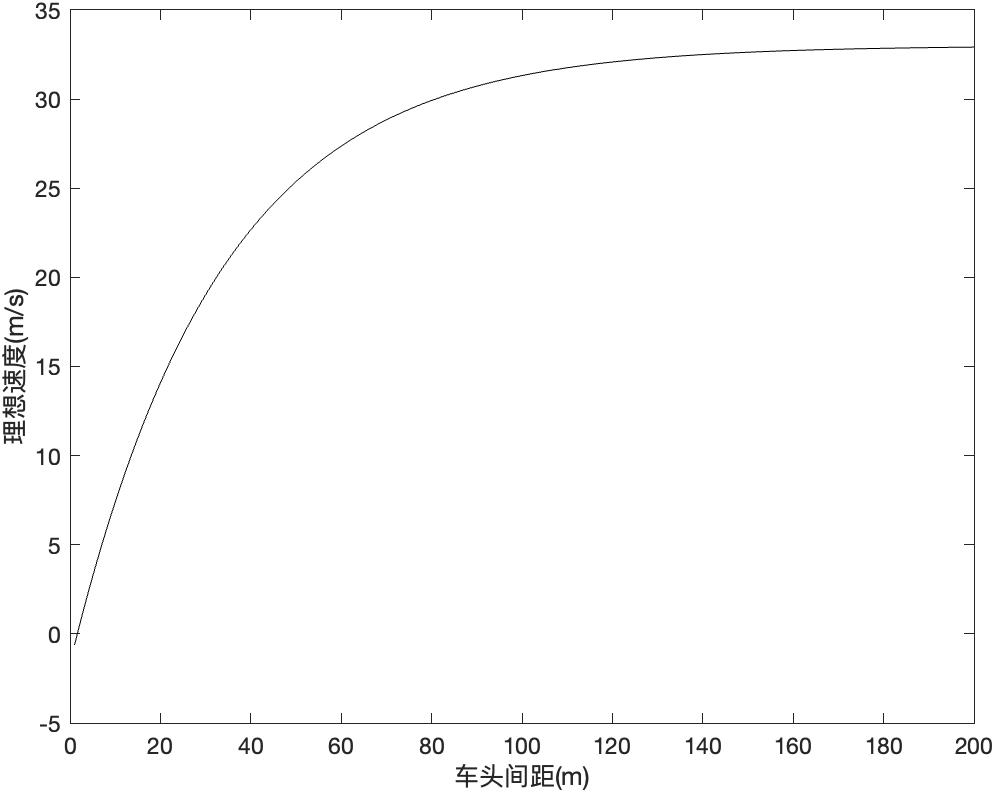
\includegraphics[width=0.45\linewidth]{chap02-2-OVM1.jpg}}
  \subcaptionbox{加速度与当前速度、车头间距的关系\label{fig:chap02-2-OVM2}}
    {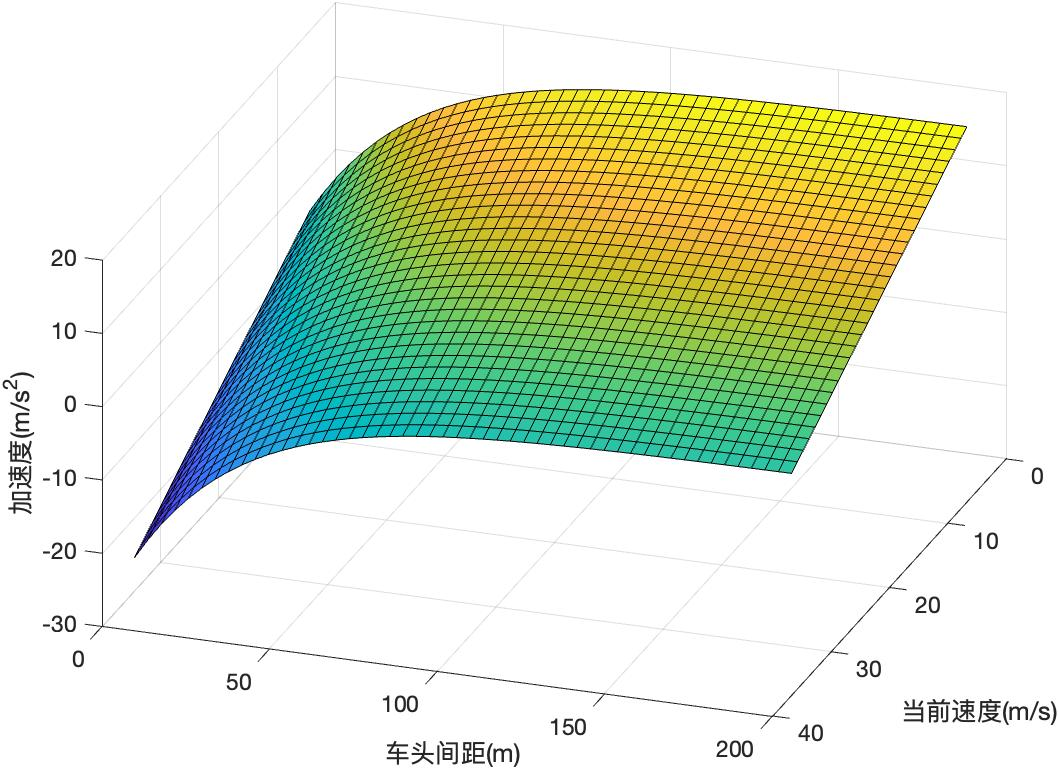
\includegraphics[width=0.5\linewidth]{chap02-2-OVM2.jpg}}
  \caption{OVM函数关系图像}
  \label{fig:chap02-2-OVM}
\end{figure}

图\ref{fig:chap02-2-OVM2}描述了车头时距、当前速度、加速度三者的关系。可以观察到当当前速度固定时,车头时距越大,加速度也越大,且呈现出与速度优化函数一样的增长规律,这与
式\ref{eq:chap02-1}是相符合的;当车头间距固定时,理想速度也就确定了,所以随着当前速度的增大,加速度线性减小。

\subsection{自动驾驶车辆跟驰模型}

自动驾驶车辆选择基于PID控制的车头时距控制算法来控制跟驰行为,该算法的表达式见式(\ref{eq:chap02-2})。
\begin{equation}
  \dot{v}_n(t) = k_1 \left[ h_n(t) - l - t_hv_n(t) \right] + k_2 \left[ v_{n-1}(t) - v_n(t) \right]
  \label{eq:chap02-2}
\end{equation}
其中,各符号含义在表\ref{tab:chap02-2}中给出,相关参数取值在表\ref{tab:chap02-added}中给出。

\begin{table}
  \centering
  \caption{基于PID控制的车头时距控制算法符号说明}
  \begin{tabular}{cc}
    \toprule
    符号          &  含义                         \\
    \midrule
    $k_1, k_2$            & 控制系数         \\
    $t_h$                 & 理想车头时距             \\
    $l$                   & 车身长度          \\
    $h_n(t)$              & 第$n$辆车在$t$时刻与前车的车头间距        \\
    $v_n(t)$              & 第$n$辆车在$t$时刻的速度 \\
    \bottomrule
  \end{tabular}
  \label{tab:chap02-2}
\end{table}

\begin{table}
  \centering
  \caption{基于PID控制的车头时距控制算法参数取值}
  \begin{tabular}{cc}
    \toprule
    参数          &  取值                         \\
    \midrule
    控制系数$k_1$          & 0.8         \\
    控制系数$k_2$          & 0.8     \\
    理想车头时距$t_h$       & $0.6s$             \\
    车身长度$l$            & $5m$         \\
    \bottomrule
  \end{tabular}
  \label{tab:chap02-added}
\end{table}

可以发现在该算法控制下,车辆的加减速由两部分控制。一是当前的两车车头距离与理想的车头距离的大小关系,如果当前两车车头距离小于理想的车头距离,那么参数$k_1$控制的部分倾向于减速;
二是当前车与前车的速度大小关系,如果当前车速度大于前车速度,$k_2$控制的部分倾向于减速。通过改变$k_1$和$k_2$的值,可以调节这两个部分的权重,二者综合即可决定当前车应当加速还是
减速,以及加速度的大小。


\section{仿真平台的搭建}
\label{sec:simulation-platform}

仿真基于MATLAB软件,模拟了一个由11辆车组成的车队,如图\ref{fig:chap02-3-simu1}所示。车队中的第一辆车是头车,其既不是人工驾驶车辆也不是自动驾驶车辆,而是按照实现规定好的策略行驶,即在0时刻以$-2m/s^2$的
加速度减速到原速度的$90\%$,紧接着以$2m/s^2$的加速度恢复元素,其速度变化情况如图\ref{fig:chap02-3-simu2}所示。如此设置头车是为了加入扰动,虽扰在真实场景下扰动可能发生在车队中的任何一辆车上,由于受到
该扰动影响的车辆是此车之后的车辆,只要将此车看作头车,就与仿真实验场景一致了,所以这样的仿真情景具有一定的一般性。

\begin{figure}
  \centering
  \subcaptionbox{车队示意图\label{fig:chap02-3-simu1}}
    {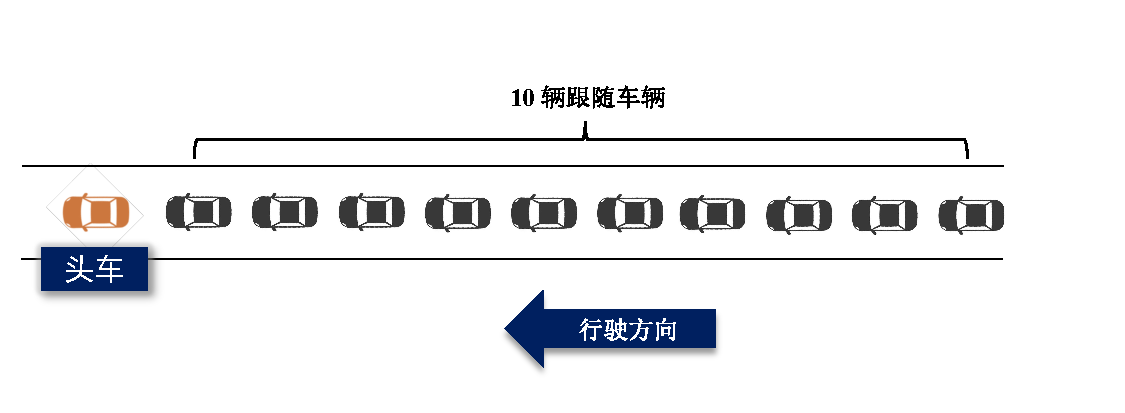
\includegraphics[width=0.7\linewidth]{chap02-3-simu1.pdf}}
  \subcaptionbox{头车速度变化曲线(初速度$20m/s$,截取前$10s$)\label{fig:chap02-3-simu2}}
    {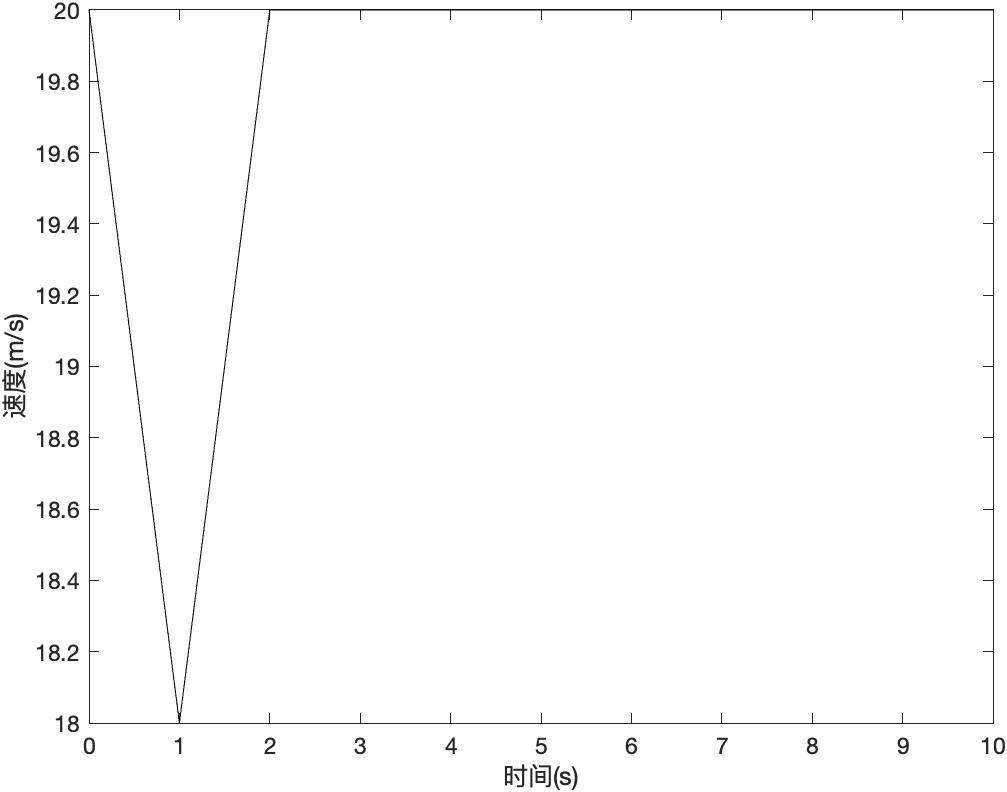
\includegraphics[width=0.6\linewidth]{chap02-3-simu2.jpg}}
  \caption{仿真场景设置}
  \label{fig:chap02-2-simu}
\end{figure}

10辆跟随车辆中自动驾驶车辆的占比为$p$($p \in [0, 1]$),在仿真过程中以$0.1$为间隔对$p$取值,当$p=0$时车队退化为纯人工驾驶车辆车队,当$p=1$时车队退化为纯自动驾驶车辆车队。

因为仿真主要关注加入的扰动对车队的影响,所以在仿真的0时刻,将车队设置为均衡状态。均衡状态的定义见定义~\ref{def:chap02-def1}。车队中的所有车辆均以均衡速度行驶。

\begin{definition}[车队的均衡状态]
  如果车队中每辆车都以相同的速度行驶,且每辆的加速度均为0,认为此时车队处于均衡状态。
  \label{def:chap02-def1}
\end{definition}

为了数值仿真不能模拟连续情况,首先将连续场景离散化。为了离散化带来的误差,实验中仿真步长取$0.01s$,总仿真时长为$500s$,这意味着有50000个采样点。

为了使仿真尽可能的接近真实情况,也应考虑实际情况中的物理限制,如真实场景下车辆的加速度大小是有限制的,这与轮胎与道路摩擦因数等因素有关。在中国智能交通协会2020年7
月发布的《基于车辆轨迹数据等汽车驾驶人驾驶行为安全性评价规范》的团体标准中,对于不同的速度区间,给出了急加速和急减速行为不同安全等级瞬间加速度的分类阈值,将安全等级
划分为安全、较安全、较危险、危险四个等级。在本工作的仿真中,车队的初始均衡速度最小不低于$10m/s$,最大不超过$30m/s$。对于急加速行为,对于$10\sim 30m/s$的速度,较危险的
加速度区间大致为$(2.7m/s^2, 4.2m/s^2)$;对于急减速行为,对于$10\sim 30m/s$的速度,较危险的加速度区间大致为$(-3.7m/^2, -2.2m/s^2)$\cite{2020safety}。
综合考虑,在仿真中将加速度限制在$[-3m/s^2, 4m/s^2]$。

另一个物理限制体现在碰撞上,在仿真过程中会出现车辆追尾的情况,在搭建仿真平台时,设置若发生碰撞,则终止当前实验。

为了使仿真更加接近真实情况,在仿真中还添加了一阶惯性环节,如式\ref{eq:chap02-added}所示,使得加速度的变化更加平滑,也更接近真实场景。
\begin{equation}
  a(t) \leftarrow 0.8a(t-1) + 0.2a(t)
  \label{eq:chap02-added}
\end{equation}

最后,考虑到人类驾驶员通过直观感受获取己车与前车的信息,也不会时时对信息的变化做出反馈,因为对于人工驾驶车辆,增加了反应延迟$\increment{t} = 1.2$秒。

对于在引言中提到的仿真过程不直观的问题,在本工作中也实现了简易的仿真过程可视化,如图\ref{fig:chap02-4-vis}所示,如此就可以直观地观察车队中车与车之间的距离大小,也可以直观
地感受潜在危险时刻和碰撞的发生。

\begin{figure}
  \centering
  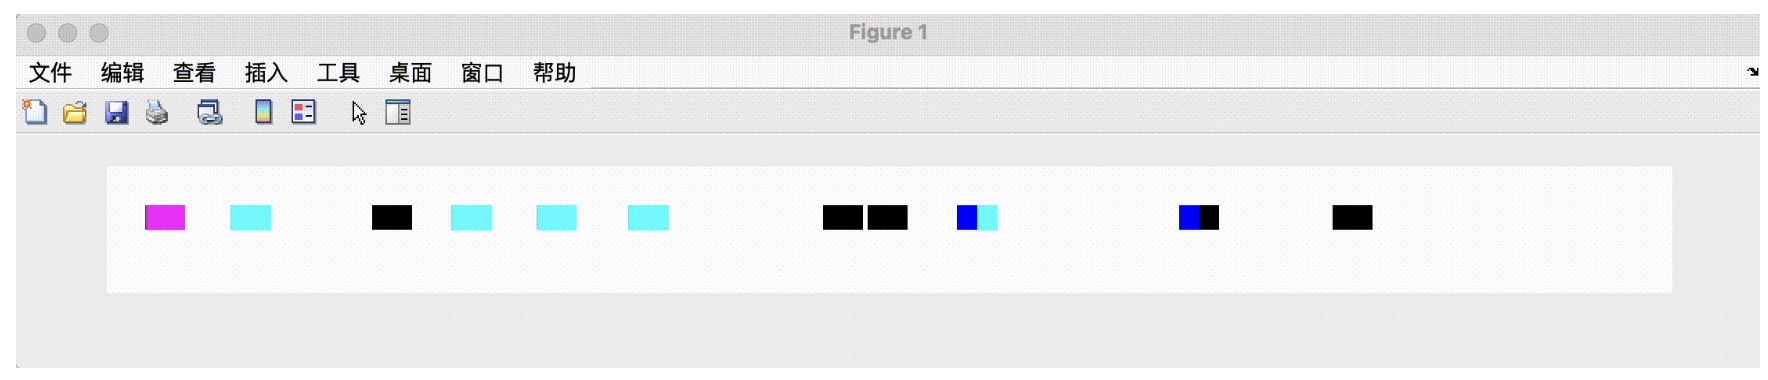
\includegraphics[width=1\linewidth]{chap02-4-vis.jpg}
  \caption*{紫色车辆为头车,浅蓝色车辆为自动驾驶车辆,黑色车辆为人工驾驶车辆,车辆前一半为深蓝色代表该车辆此时刻存在潜在危险}
  \caption{仿真过程可视化}
  \label{fig:chap02-4-vis}
\end{figure}

表\ref{tab:chap02-3}列出了仿真平台的重要参数取值。

\begin{table}
  \centering
  \caption{仿真平台重要参数取值}
  \begin{tabular}{cc}
    \toprule
    参数                   &  取值                         \\
    \midrule
    仿真步长                & 0.01$s$         \\
    仿真时常                & $500s$             \\
    车辆总数                & 11              \\
    初始均衡速度取值区间      & $[10m/s, 30m/s]$        \\
    车辆加速度最小值         & $-3m/s^2$     \\
    车辆加速度最大值         & $4m/s^2$ \\
    人类驾驶员反应延迟       & $1.2s$ \\
    \bottomrule
  \end{tabular}
  \label{tab:chap02-3}
\end{table}

\section{仿真平台真实性分析}

首先对车辆加速度的仿真情况进行分析,在\ref{sec:2.2}中介绍了车辆的跟驰模型,但可以发现无论是人工驾驶车辆还是自动驾驶车辆都没有对加速度的大小做出限制,通过
图\ref{fig:chap02-2-OVM2}可以发现人工驾驶车辆的加速度甚至出现了小于$-15m/s^2$、大于$15m/s^2$的情况,这显然是不合理的。这也是在\ref{sec:simulation-platform}
中对仿真过程中车辆加速度的大小进行了限制的原因,下面限制前后的仿真情况进行分析。

\begin{figure}
  \centering
  \subcaptionbox{限制加速度前加速度曲线\label{fig:chap02-5-a-0.7-15-fig}}
    {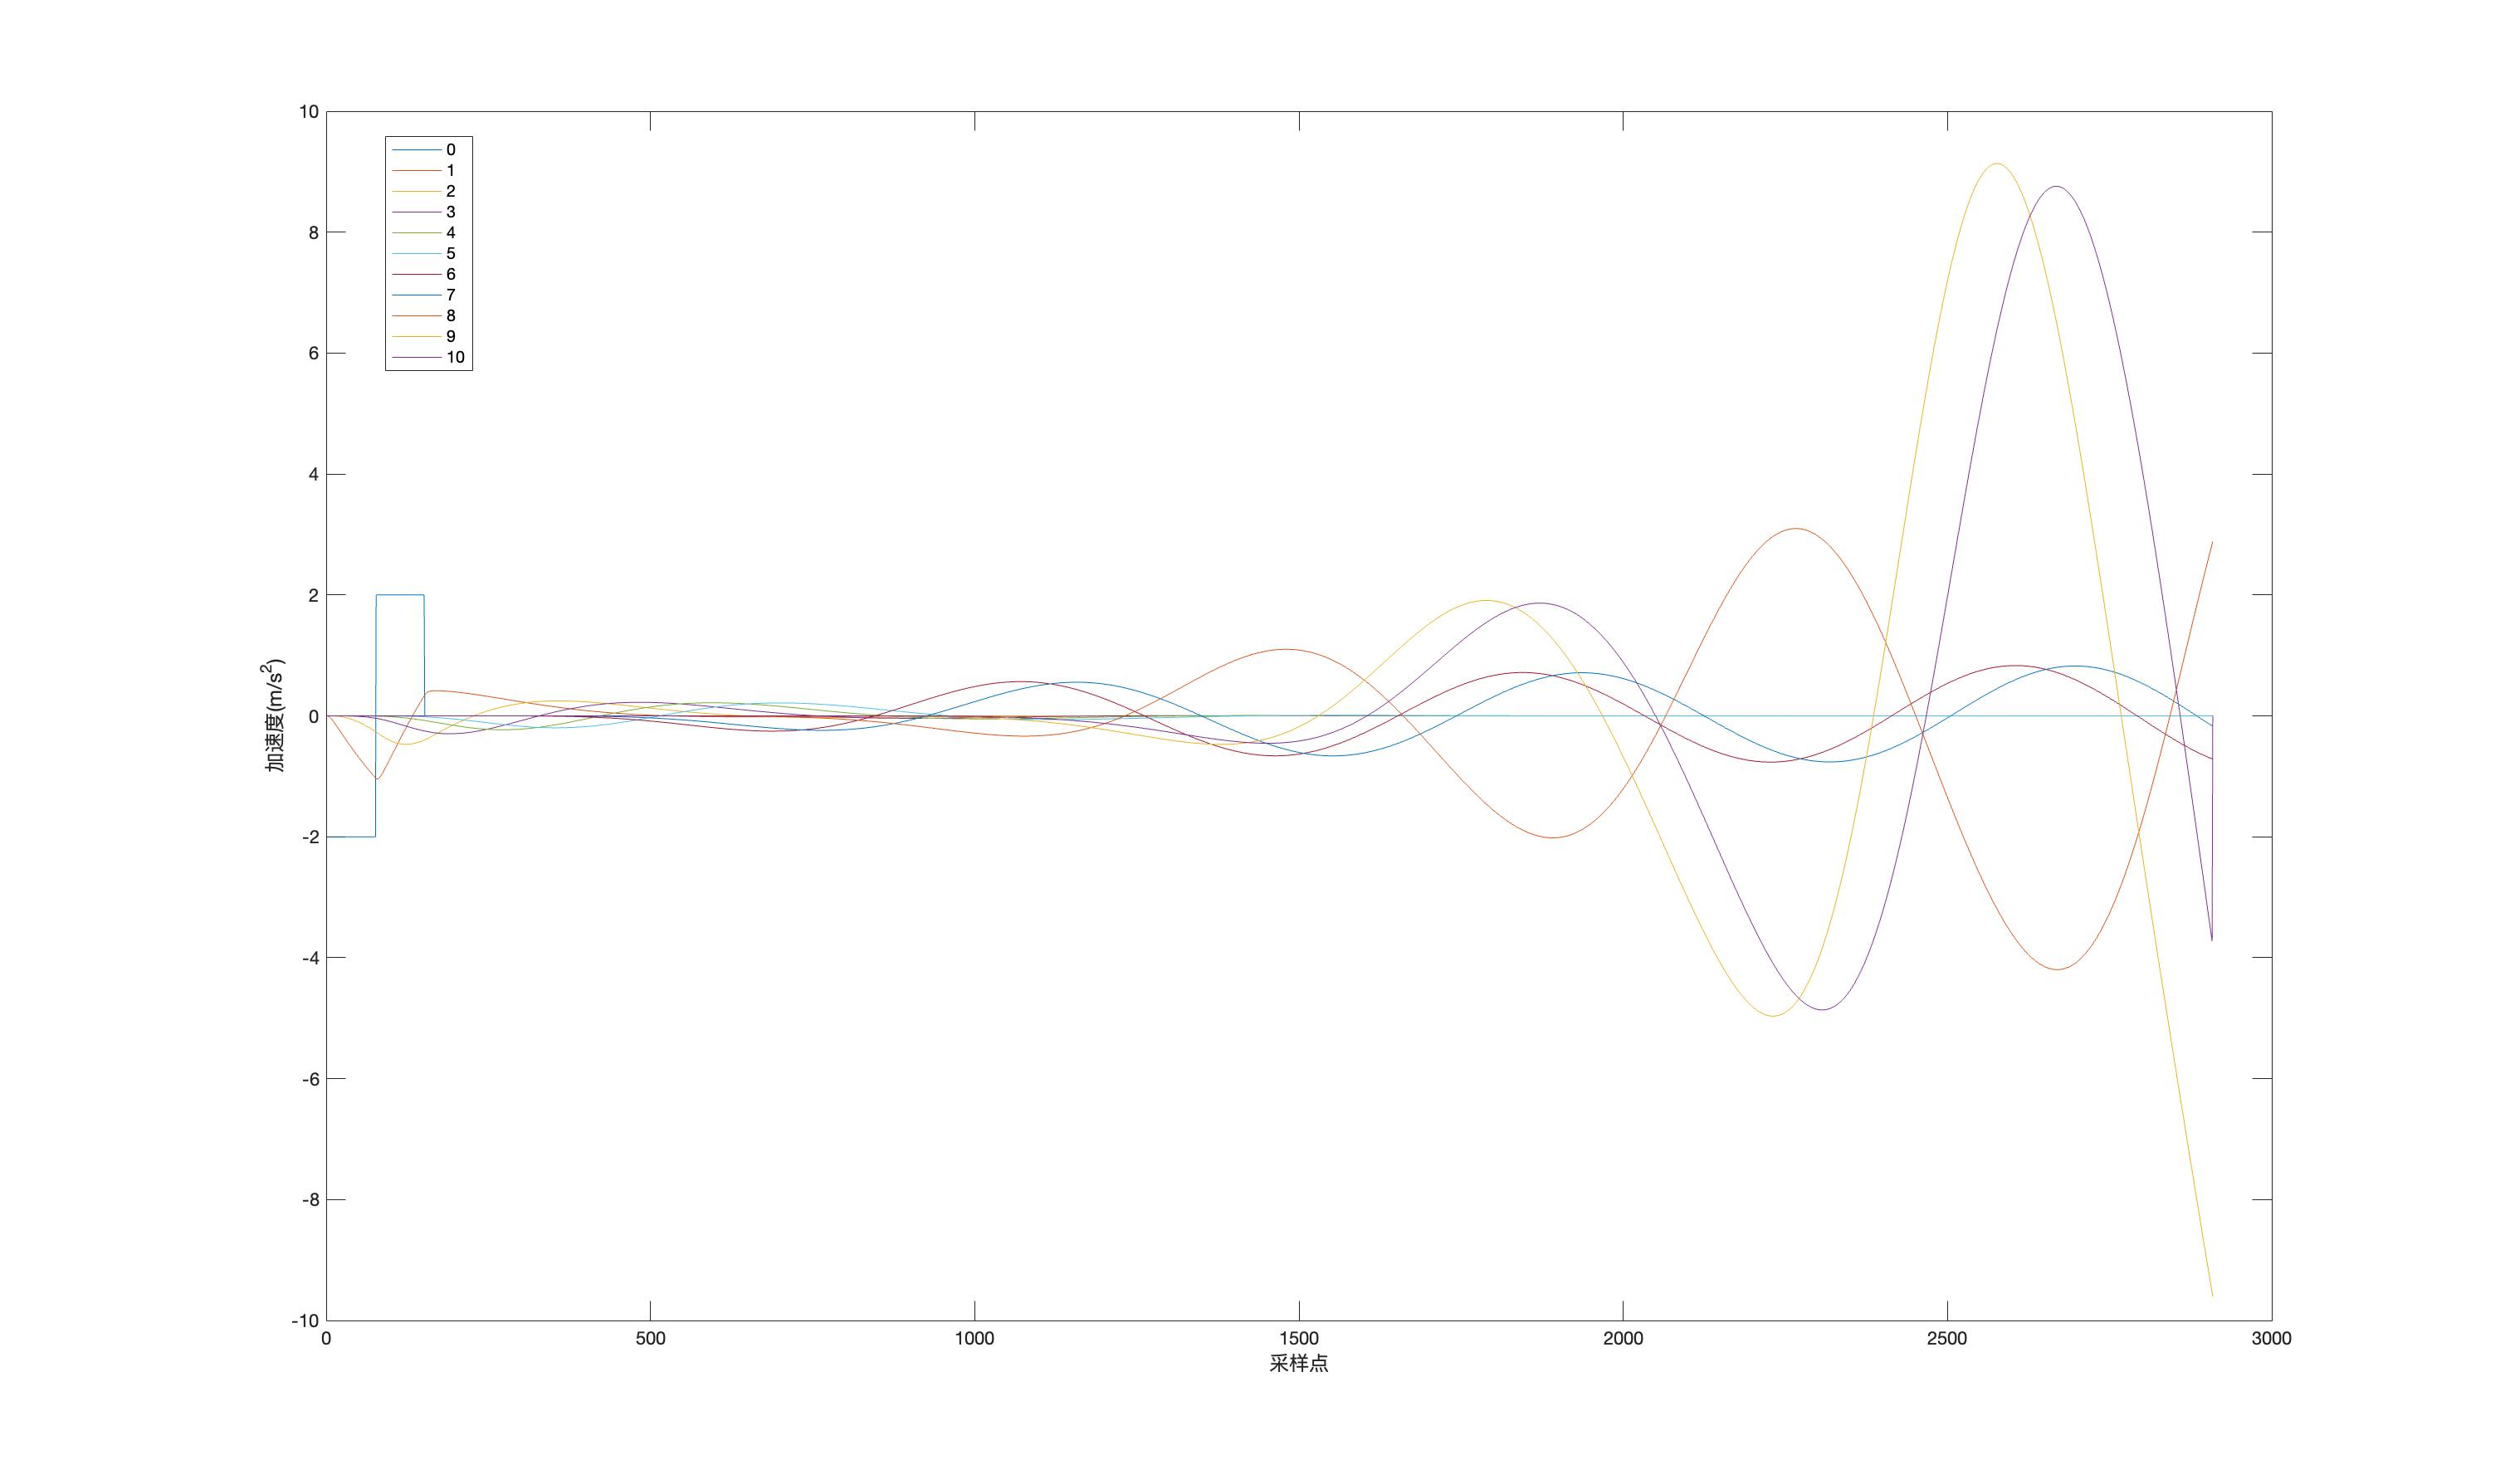
\includegraphics[width=0.55\linewidth]{chap02-5-a-0.7-15-fig.jpg}}
  \subcaptionbox{限制加速度前加速度分布\label{fig:chap02-5-a-0.7-15-his}}
    {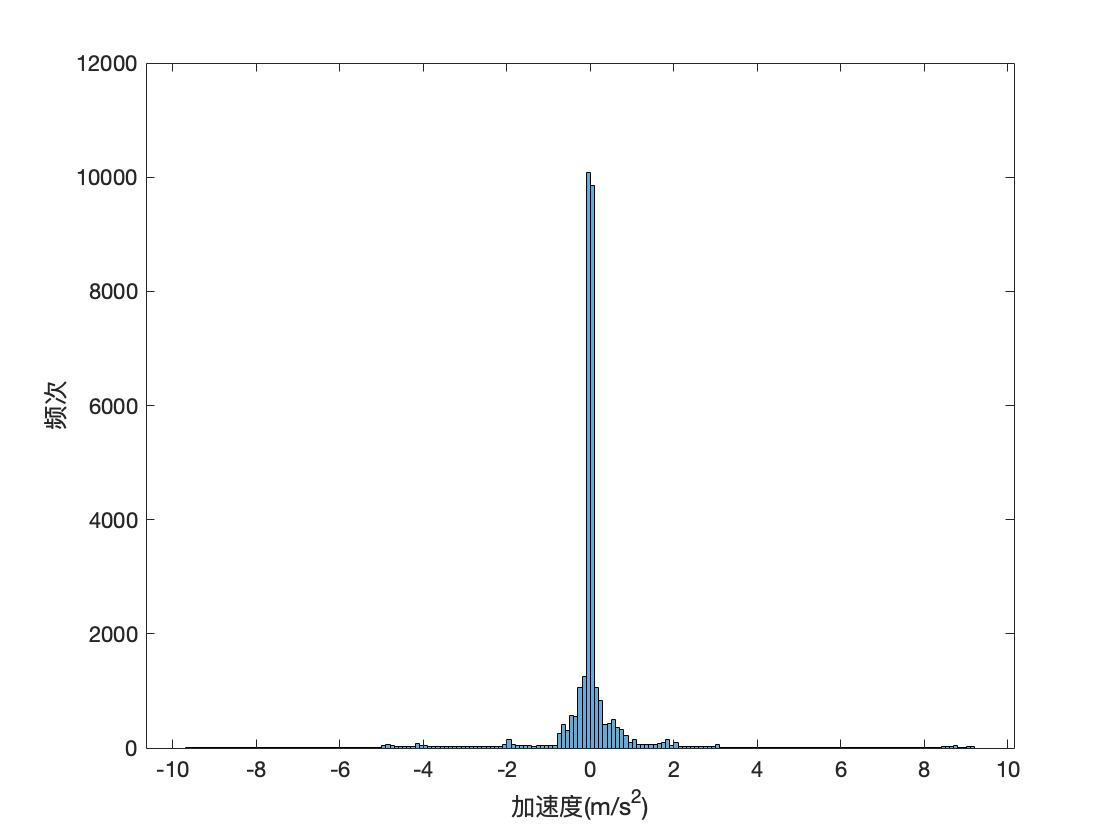
\includegraphics[width=0.4\linewidth]{chap02-5-a-0.7-15-his.jpg}}
  \subcaptionbox{限制加速度后加速度曲线\label{fig:chap02-5-a-0.7-15-limited-fig}}
    {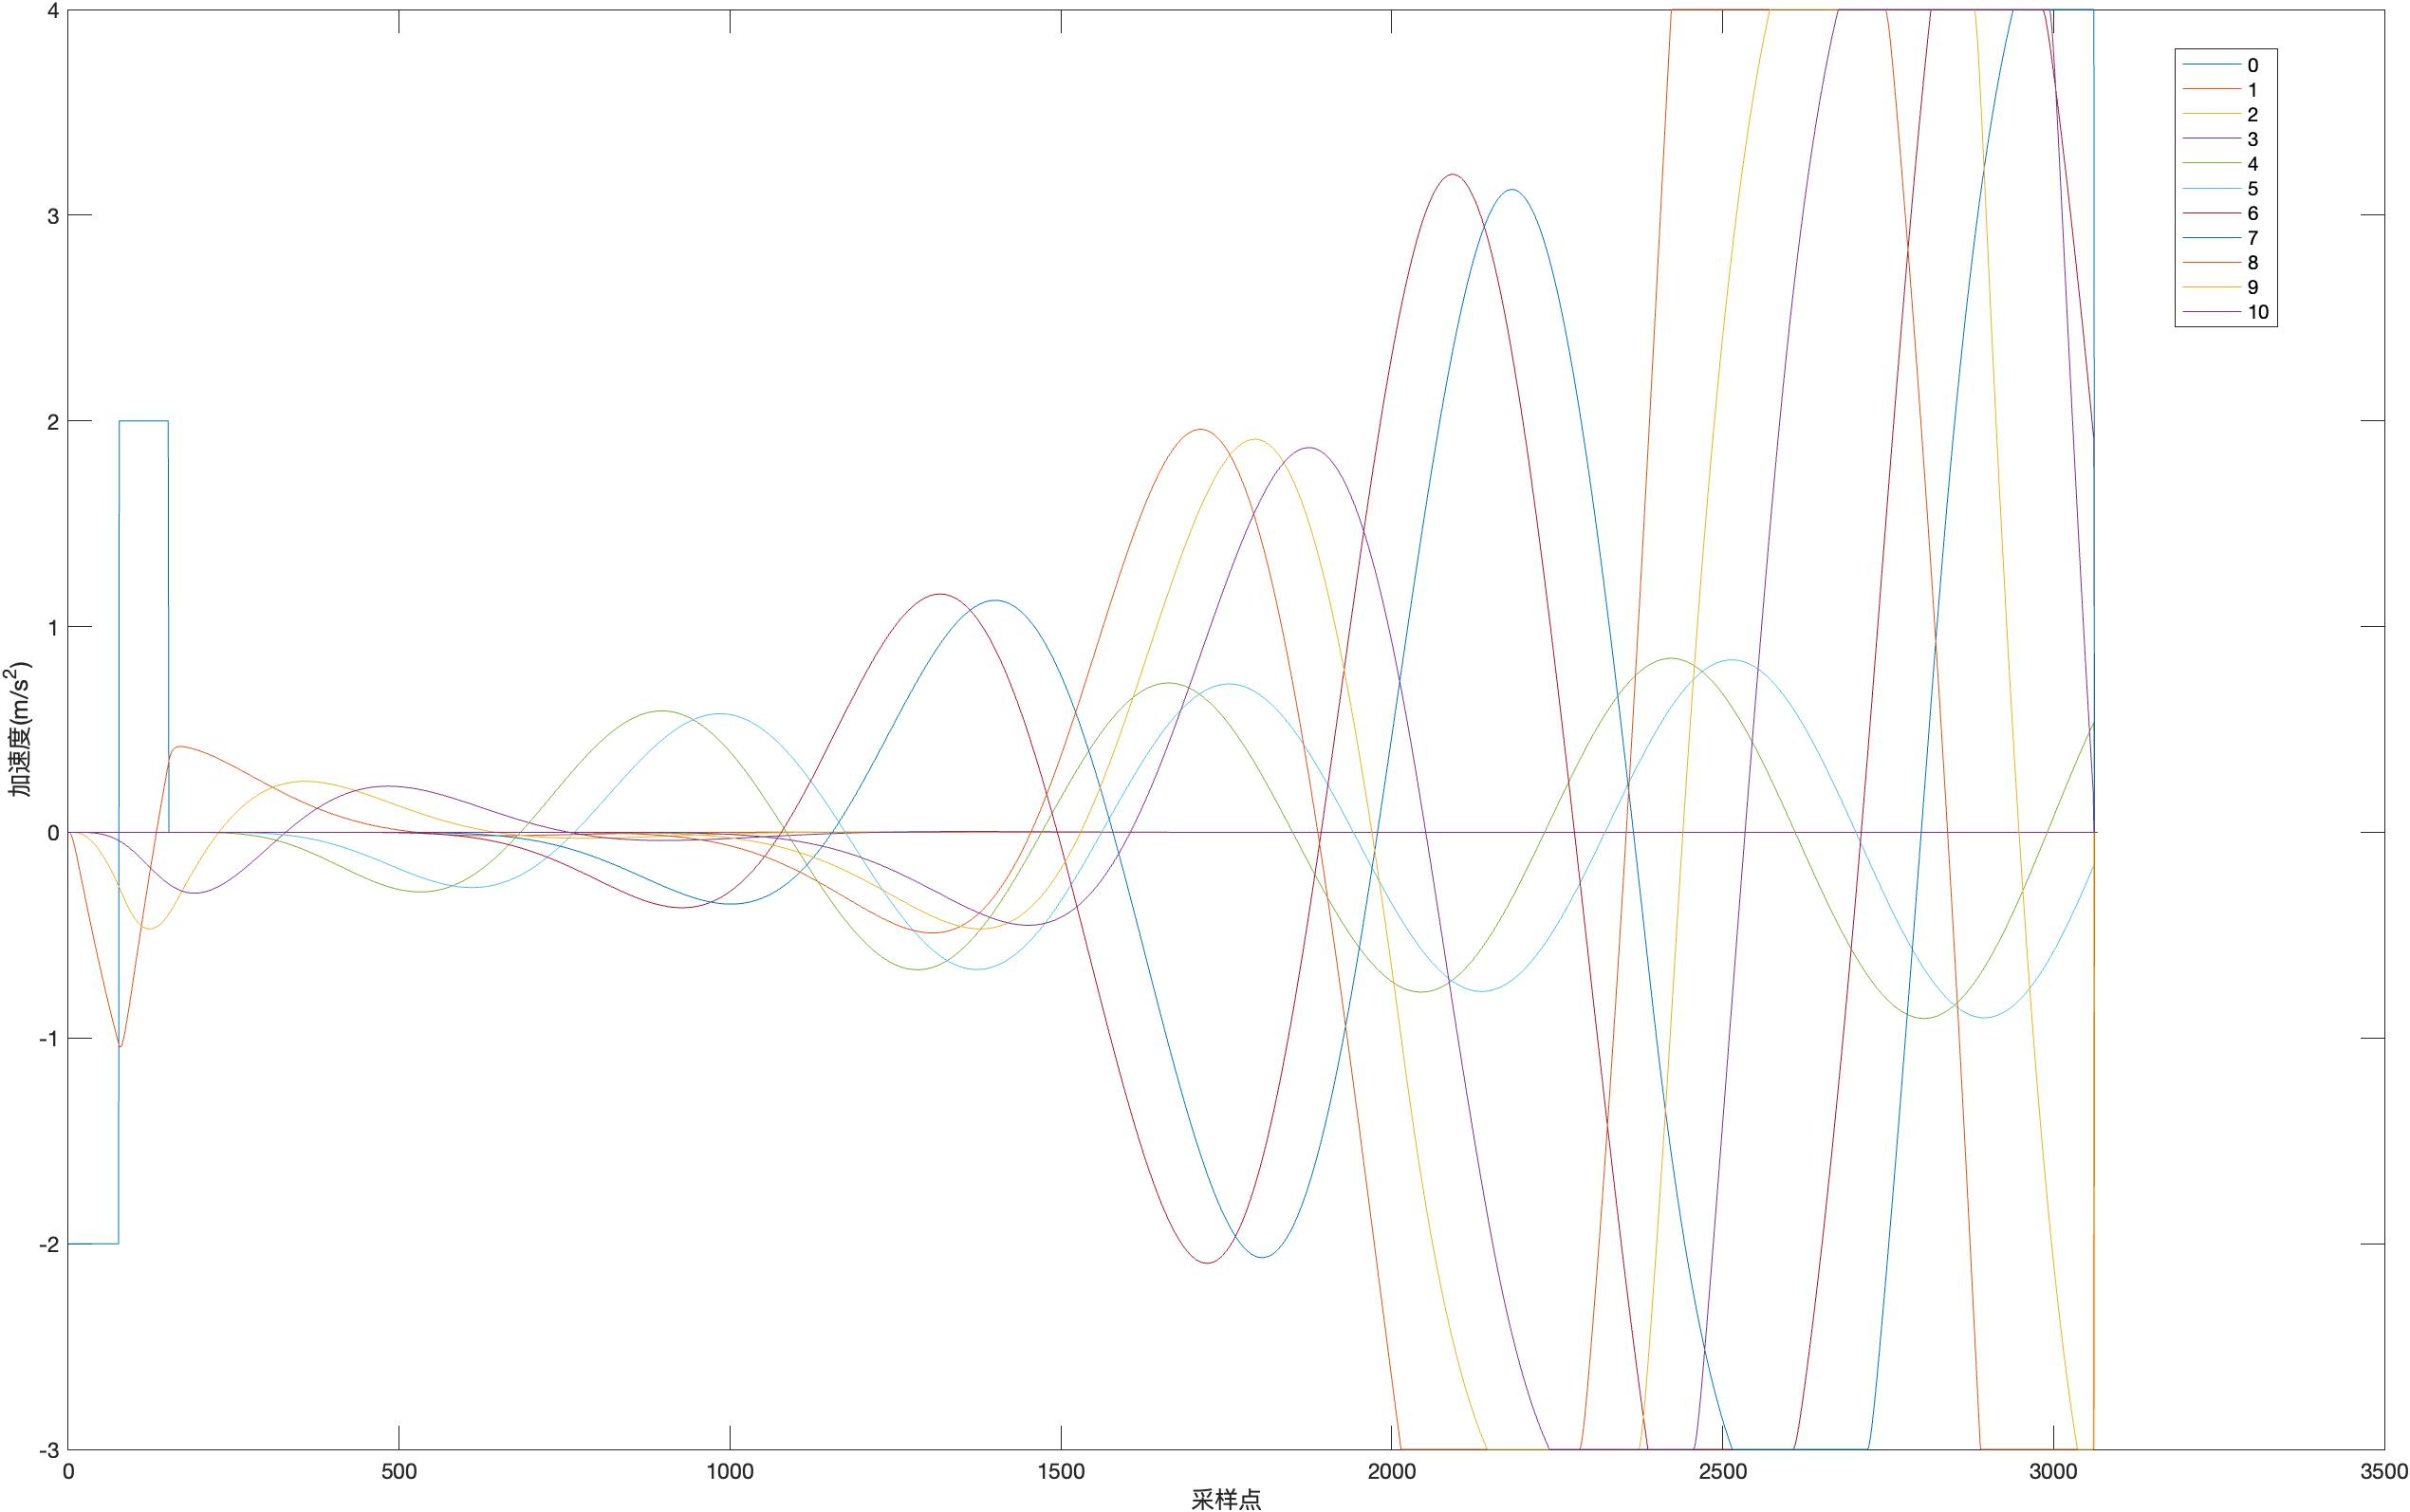
\includegraphics[width=0.45\linewidth]{chap02-5-a-0.7-15-limited-fig.jpg}}
\subcaptionbox{限制加速度后加速度分布\label{fig:chap02-5-a-0.7-15-limited-his}}
    {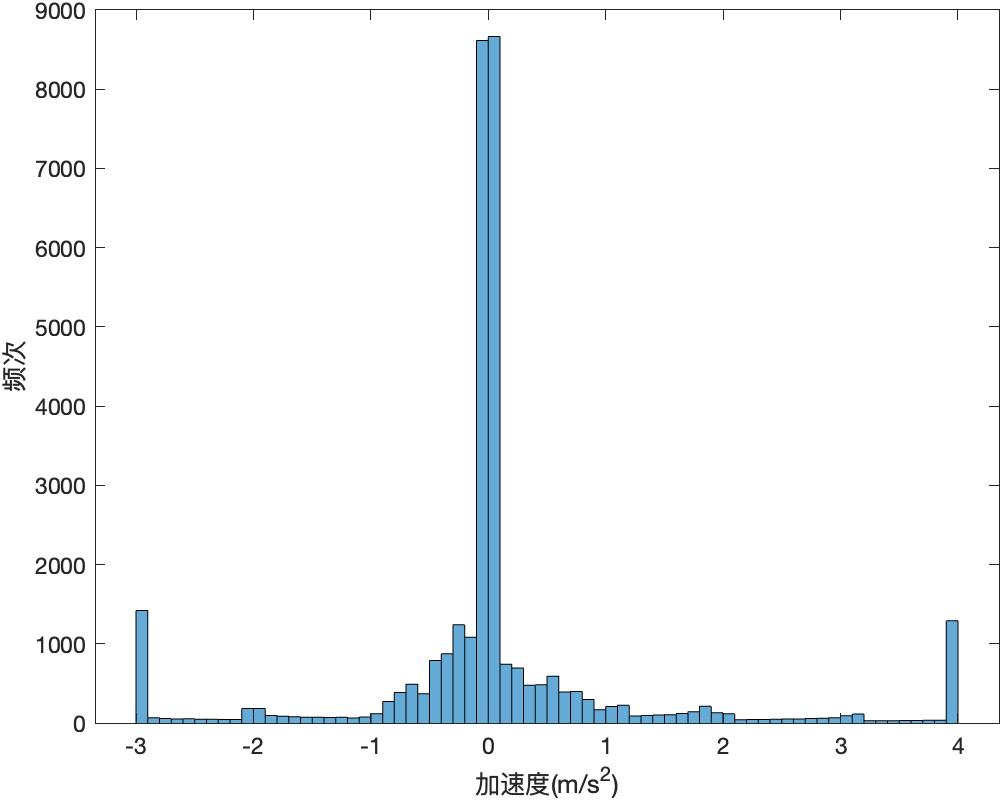
\includegraphics[width=0.35\linewidth]{chap02-5-a-0.7-15-limited-his.jpg}}
  \caption{车队不稳定时仿真过程中加速度情况}
  \label{fig:chap02-5-a}
\end{figure}

当自动驾驶车辆比例为$0.7$,初始均衡速度为$15m/s$时,车队处于不稳定的状态(将在第\ref{sec:3}章进行介绍)。图\ref{fig:chap02-5-a-0.7-15-fig}和
\ref{fig:chap02-5-a-0.7-15-his}描述了对加速度大小进行限制前,加速度曲线和加速度分布情况。

可以发现在仿真过程中,加速度存在接近$\pm 10m/s$的情况,这是不合理的。图\ref{fig:chap02-5-a-0.7-15-limited-fig}和\ref{fig:chap02-5-a-0.7-15-limited-his}
描述了限制加速度大小之后加速度曲线和加速度分布情况。对于不稳定的车队,扰动会逐渐增大,存在较多的加速度边界值是比较合理的。

\begin{figure}
  \centering
  \subcaptionbox{限制加速度后加速度曲线 \label{fig:chap02-6-a-fig}}
    {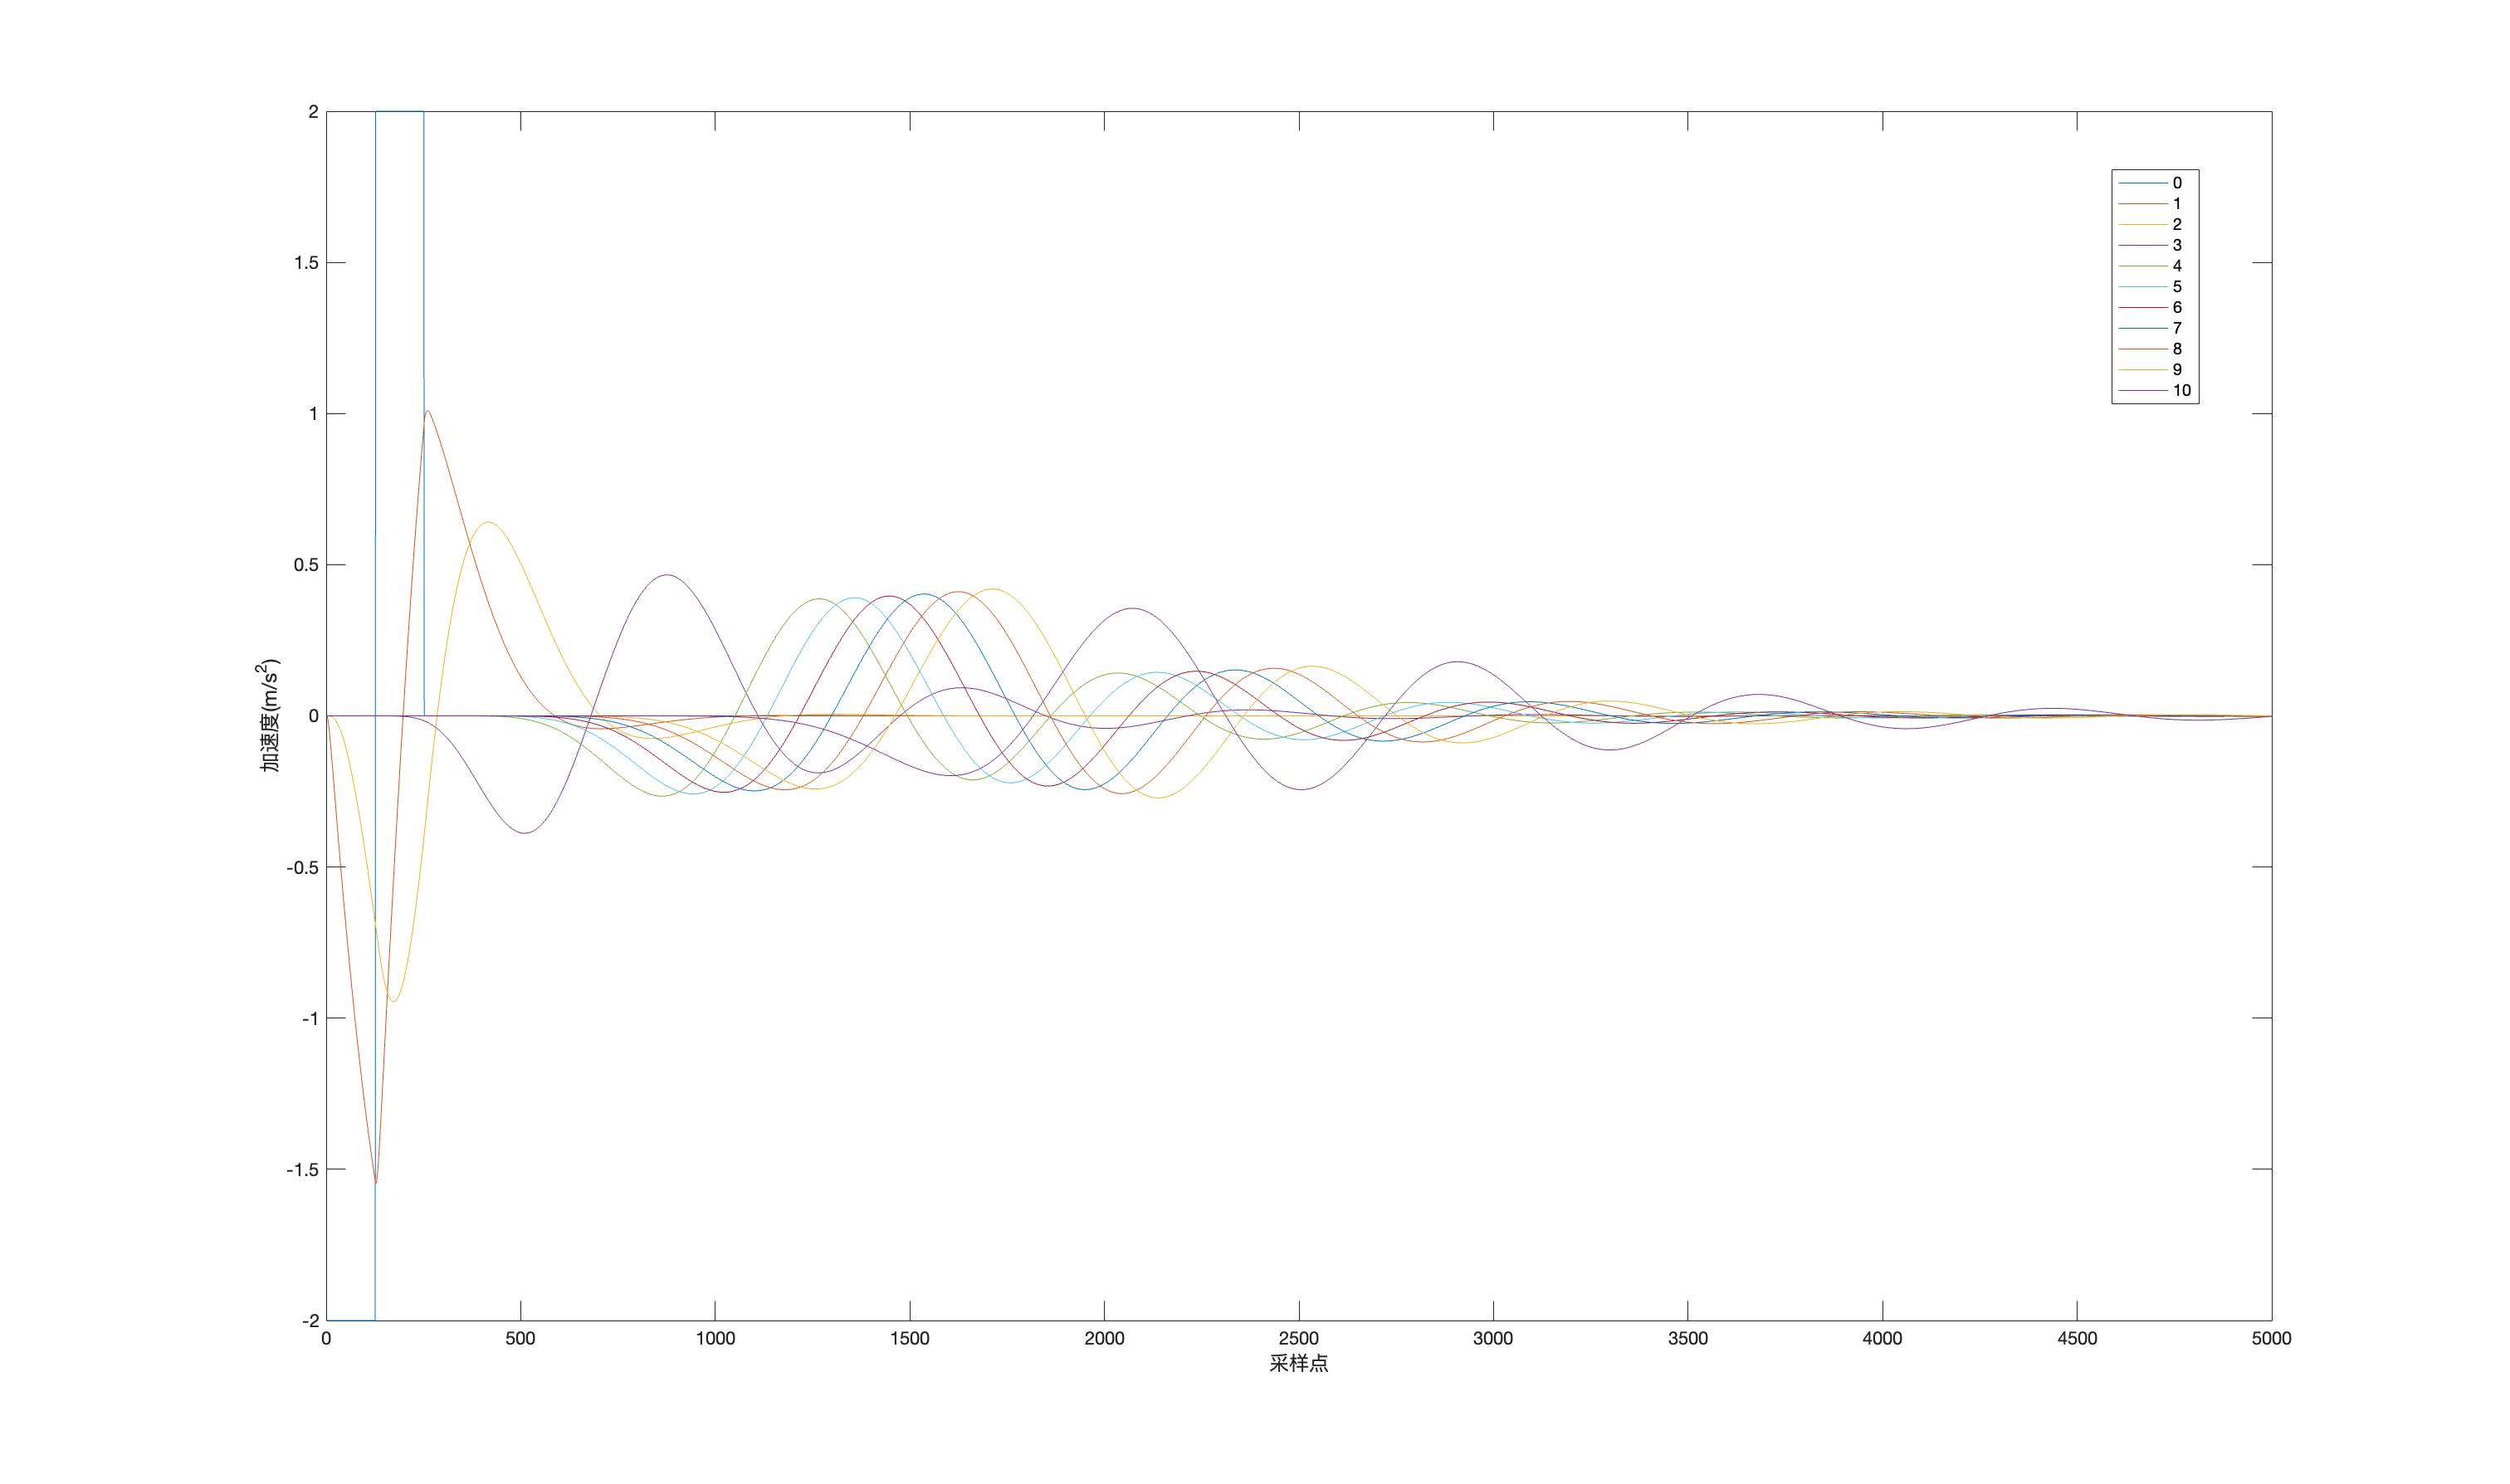
\includegraphics[width=0.55\linewidth]{chap02-5-a-0.7-25-limited-fig.jpg}}
  \subcaptionbox{限制加速度后加速度分布 \label{fig:chap02-6-his}}
    {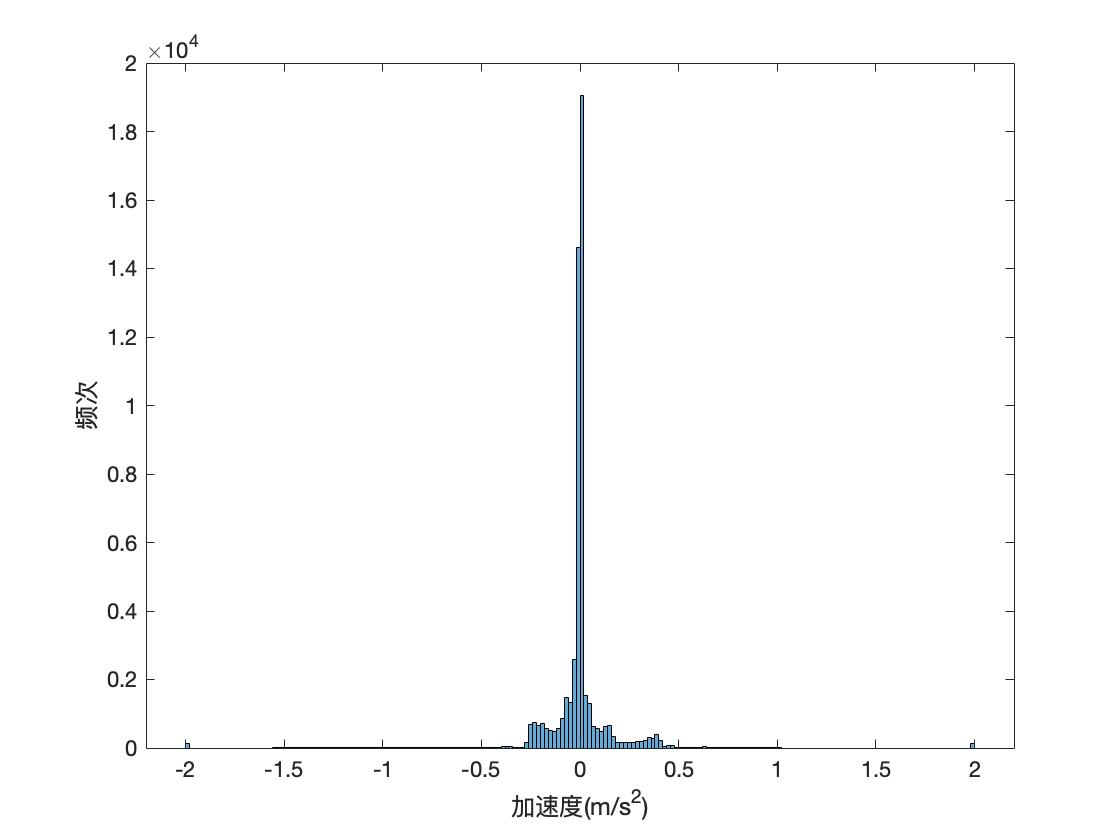
\includegraphics[width=0.4\linewidth]{chap02-5-a-0.7-25-limited-his.jpg}}
    \caption{车队稳定时仿真过程中加速度情况}
  \label{fig:chap02-6}
\end{figure}

对于处于稳定状态的车队,如自动驾驶车辆比例为$0.7$,初始均衡速度为$25m/s$,其加速度情况如图\ref{fig:chap02-6}所示。

可以观察到加速度大小主要集中在$[-0.5m/s^2, 0.5m/s^2]$,这与实际交通情况较相符。

对于仿真过程中车辆的速度情况,也通过自动驾驶车辆比例为$0.7$时,初始均衡速度为$15m/s$和$25m/s$两种情况来简单验证。

\begin{figure}
  \centering
  \subcaptionbox{初始均衡速度为$15m/s$ \label{fig:chap02-7-a-fig}}
    {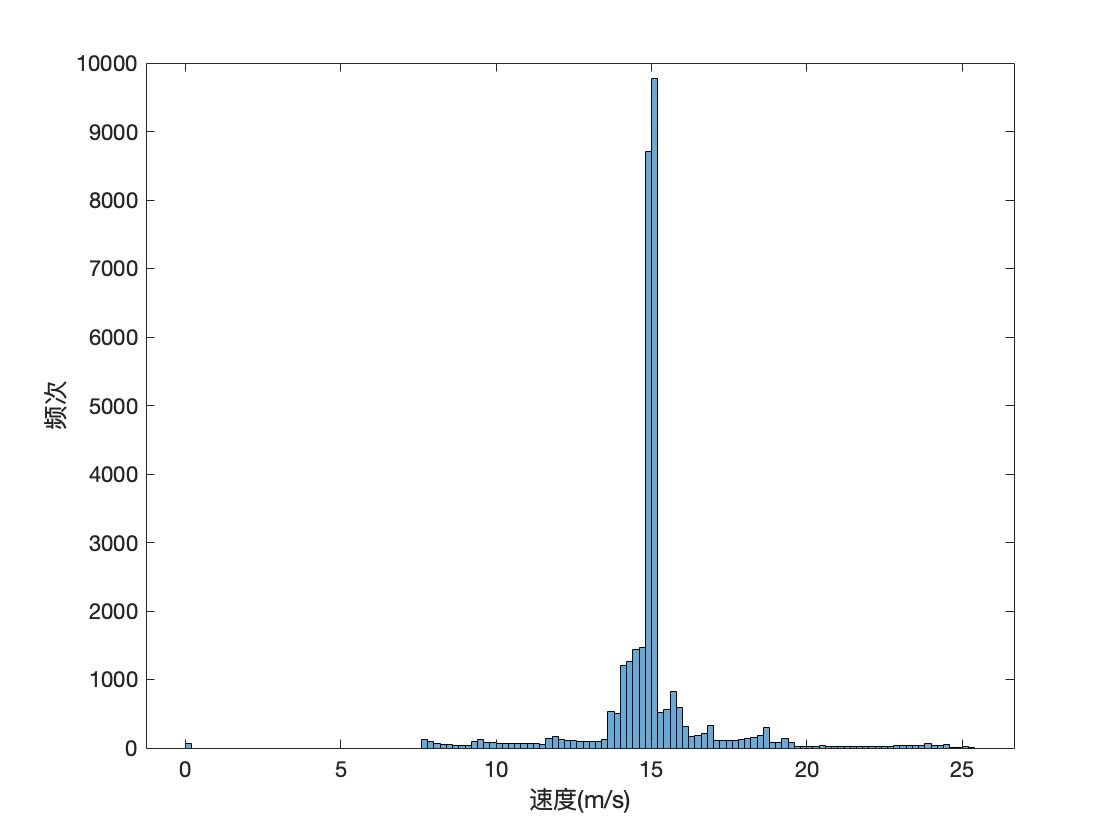
\includegraphics[width=0.45\linewidth]{chap02-5-v-0.7-15-limited-his.jpg}}
  \subcaptionbox{初始均衡速度为$25m/s$ \label{fig:chap02-7-his}}
    {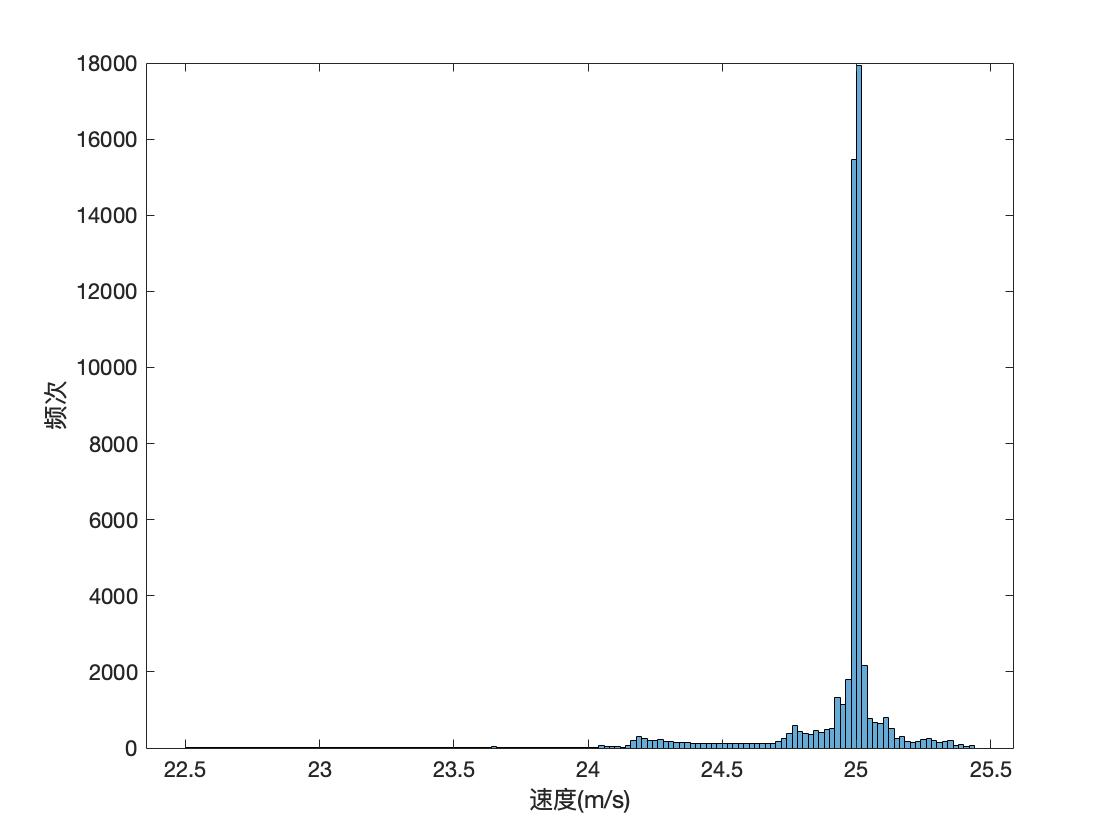
\includegraphics[width=0.45\linewidth]{chap02-5-v-0.7-25-limited-his.jpg}}
  \caption*{自动驾驶车辆比例为$0.7$}
  \caption{仿真过程中速度情况}
  \label{fig:chap02-7}
\end{figure}

由于已经通过限制使得加速度大小处于合理的区间,即速度的变化快慢已经较为合理,还需要验证速度分布的合理性。如图\ref{fig:chap02-7}所示两种情况下速度大小均主要分布在初始
均衡速度附近,且取值均合理。

\section{本章小结}

本章介绍了仿真平台的搭建,并对仿真平台的真实性进行分析。仿真平台中的车辆是根据其跟驰策略行驶的,在本章中首要介绍了人工驾驶车辆和自动驾驶车辆选用
的跟驰模型;接着简要介绍了仿真所用的平台以及仿真的参数;最后,由于仿真的真实性将直接影响本工作的实际意义,所以在本章中对仿真的真实性进行了分析。

本章的结构如图\ref{fig:chap02-1-logic}所示。

\begin{figure}
  \centering
  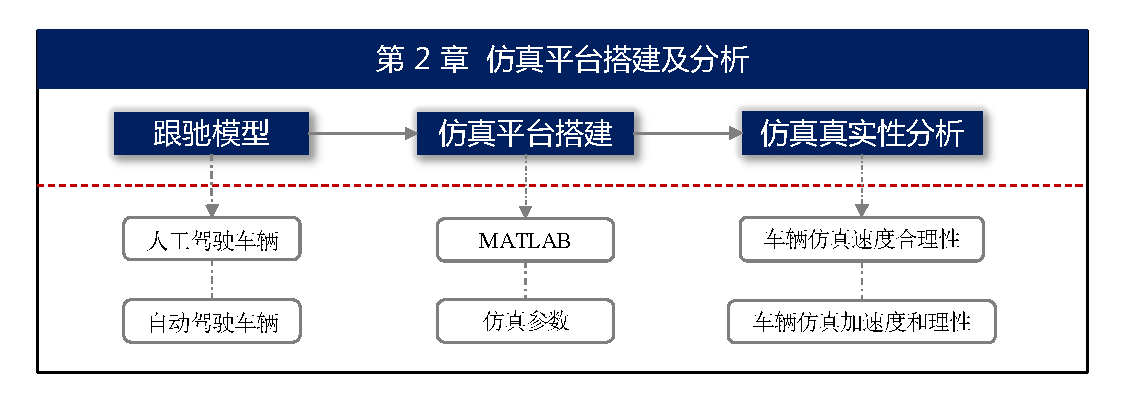
\includegraphics[width=1\linewidth]{chap02-1-structure.pdf}
  \caption{第2章结构}
  \label{fig:chap02-1-logic}
\end{figure}